\documentclass[12pt,a4paper]{book} 
\usepackage[margin=0.8in]{geometry}
\usepackage[portuguese]{babel}
\usepackage{pgffor}
\usepackage{xcolor}
\usepackage{tikz}
\usepackage{graphicx}

\pagenumbering{Roman}

\usepackage{fancyhdr}

\pagestyle{fancyplain}
\fancyhead[L]{}
\fancyhead[C]{\textbf{\thepage}}
\fancyhead[R]{}
\fancyfoot[L]{}
\fancyfoot[C]{}
\fancyfoot[R]{}


\newcommand{\face}[2]{
    \begin{titlepage}
        \topskip0pt
        \vspace*{\fill}
        \begin{center}
            \textbf{\Huge{#1} \\ \uppercase{\large{#2}}}
        \end{center}
        \vspace*{\fill}
    \end{titlepage}
}

\newcommand{\guitarneck}{
    \resizebox{1.9cm}{!}{
        \begin{tikzpicture}
            \tikzstyle{every node}=[font=\LARGE]
            \draw (3.75,17.75) to[short] (8.75,17.75);
            \draw (3.75,16.5) to[short] (8.75,16.5);
            \draw (3.75,15.25) to[short] (8.75,15.25);
            \draw (3.75,14) to[short] (8.75,14);
            \draw (3.75,12.75) to[short] (8.75,12.75);
            \draw [ line width=0.6pt](3.75,19) to[short] (8.75,19);
            \draw [ line width=0.6pt](8.75,19) to[short] (8.75,12.75);
            \draw [ line width=0.6pt](7.75,19) to[short] (7.75,12.75);
            \draw [ line width=0.6pt](3.75,19) to[short] (3.75,12.75);
            \draw [ line width=0.6pt](5.75,19) to[short] (5.75,12.75);
            \draw [ line width=0.6pt](4.75,19) to[short] (4.75,12.75);
            \draw [ line width=0.6pt](6.75,19) to[short] (6.75,12.75);
            \node [font=\LARGE] at (3.75,12.25) {\textbf{E}};
            \node [font=\LARGE] at (4.75,12.25) {\textbf{A}};
            \node [font=\LARGE] at (5.75,12.25) {\textbf{D}};
            \node [font=\LARGE] at (6.75,12.25) {\textbf{G}};
            \node [font=\LARGE] at (7.75,12.25) {\textbf{B}};
            \node [font=\LARGE] at (8.75,12.25) {\textbf{E}};
            \draw [ line width=0.6pt](3.75,19.25) to[short] (8.75,19.25);
        \end{tikzpicture}
    }
}

\newcommand{\mychapter}[1]{
    \newpage
    \topskip0pt
    \vspace*{\fill}
    \addtocounter{chapter}{1}
    \begin{center}
        \textbf{\Large{Capítulo Nº. \thechapter \\ \vspace{0.5cm} \uppercase{#1}}}
    \end{center}
    \vspace*{\fill}
    \newpage
    \addcontentsline{toc}{chapter}{#1}
}


\begin{document}
    \face{Livro I}{Cifras, Letras \& Acordes}

    \mychapter{Letras \& Cifras}

    \foreach \i in {1,...,60}{
        \flushleft
        \textbf{Nome:} \hrulefill
        \flushleft
        \textbf{Ano:} \rule{2cm}{0.4pt} \hspace{0.2cm} \textbf{Artista:} \hrulefill
        \flushleft
        \textbf{Pág. Acordes Violão:} \hrulefill \hspace{0.2cm} \textbf{Pág. Acordes Piano:} \hrulefill 

        \foreach \j in {1,...,13}{
            \flushleft
            \color{lightgray}
            C\j \hspace{0.2cm} \hrulefill \newline \vspace{-.5cm}
            
            \flushleft
            \color{gray}
            L\j \hspace{0.2cm} \hrulefill \newline \vspace{-.5cm}
        }
    }

    \mychapter{Acordes de Violão}
    
    \foreach \i in {1,...,40}{
        \flushleft
        \textbf{Nome:} \hrulefill 
        
        \flushleft
        \textbf{Pág. Cifra:} \hrulefill \newline

        \begin{centering}
            \foreach \j in {1,...,7}{
                \flushleft
                \foreach \k in {1,...,5}{
                    \guitarneck
                    \hspace{0.5cm}
                }
                \guitarneck
                \vspace{0.5cm}
            }
            \newpage
        \end{centering}
    }

    \mychapter{Acordes de Piano}

    \foreach \i in {1,...,40}{
        \flushleft
        \textbf{Nome:} \hrulefill 
        
        \flushleft
        \textbf{Pág. Cifra:} \hrulefill \newline

        \begin{centering}
            \foreach \j in {1,...,10}{
                \flushleft
                \foreach \k in {1,...,2}{
                    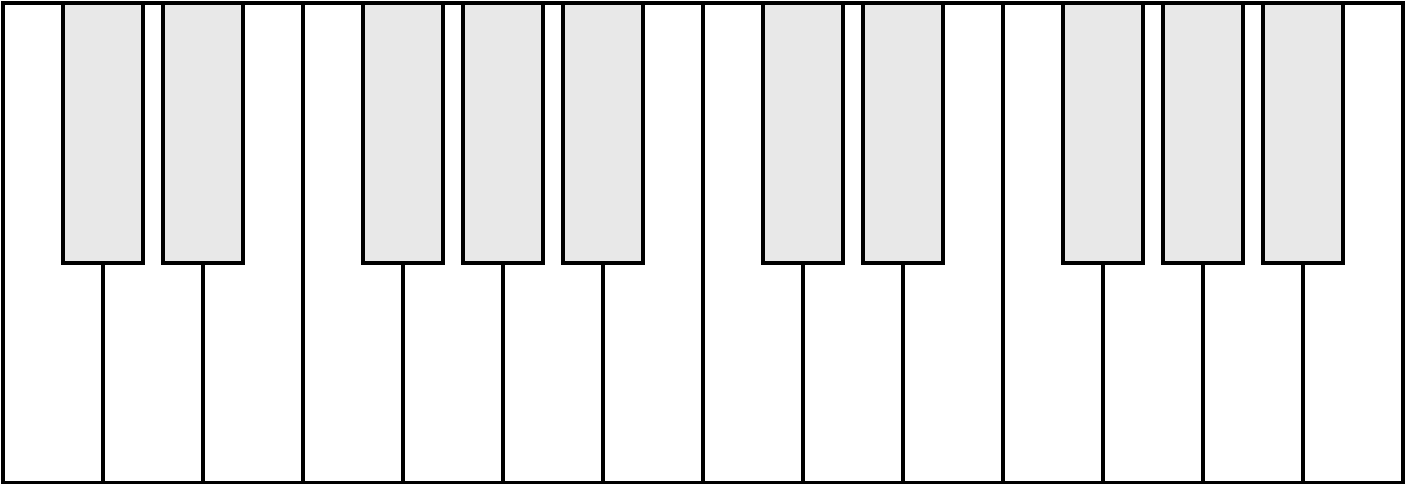
\includegraphics[width=4.5cm]{fig/piano_template.png}
                    \hspace{0.5cm}
                }
                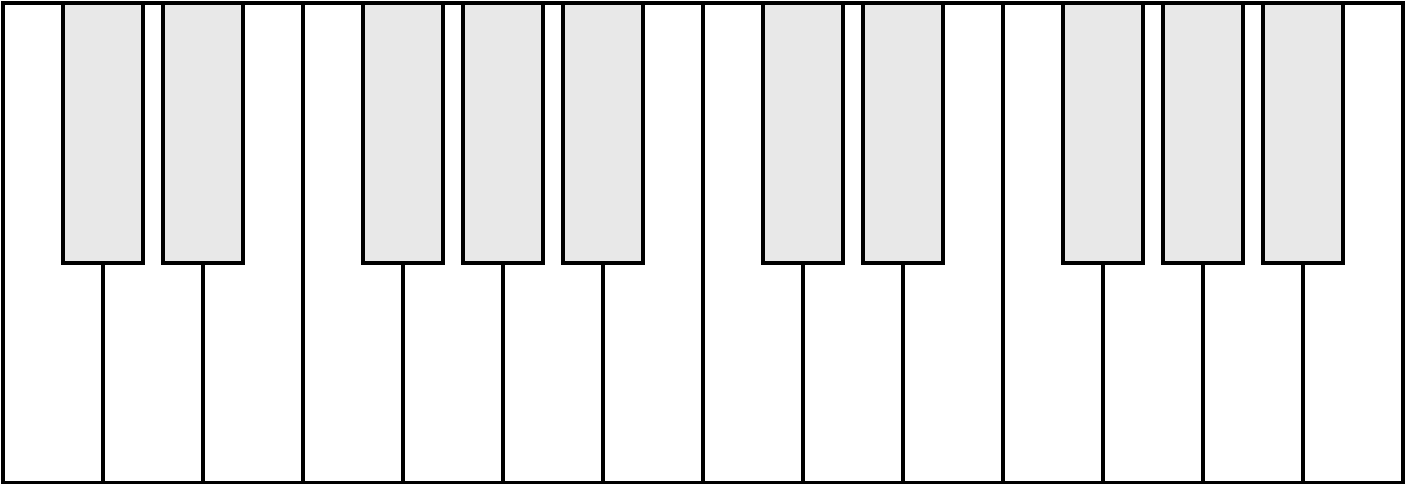
\includegraphics[width=4.5cm]{fig/piano_template.png}
                \vspace{0.5cm}
            }
            \newpage
        \end{centering}
    }

\end{document}
